\chapter{Fall degrees of point-decomposition systems}\label{ch:falldegree}

Every claim that elliptic-curve index calculus can be subexponential rests
on the cost of solving the point-decomposition system. In practice that
means its \emph{solving degree}: the largest degree a Gröbner-basis
computation reaches. Petit and Quisquater~\cite{petit2012} conjectured that
the solving degree stays close to the \emph{first fall degree}, which is
small and easy to compute. Semaev~\cite{semaev2015} assumed it is at
most 4 for his chained systems. Kosters and Yeo~\cite{kosters2015notes},
Huang, Kosters and Yeo~\cite{hky2015} and Kousidis and
Wiemers~\cite{kousidis2019} gave reasons and experiments to doubt this. All
three name rigorous bounds on the \emph{last} fall degree, which equals the
solving degree for the systems that matter, as the open problem.

This chapter collects what the programme proved and certified about these
degrees, in three presentations of the decomposition system:
\begin{itemize}
\item binary Weil descent;
\item explicit membership over any field;
\item prime-field Kummer towers.
\end{itemize}
The message is the same in all three. The first fall degree is a constant
of the presentation, whereas the last fall degree is not. Where the last
fall degree rises above 4, the chapter gives a certificate that a separate
program checks without trusting the producer.

\section{Definitions}\label{sec:fd-defs}

Let $F=\{f_1,\ldots,f_M\}\subset R=k[x_1,\ldots,x_N]$, graded by total
degree.
\begin{itemize}
\item \emph{Closure.} $V_{F,d}$ is the smallest $k$-subspace of $R_{\le d}$
  that contains $F\cap R_{\le d}$ and is closed under $g\mapsto hg$
  whenever $\deg(hg)\le d$~\cite{hky2015,caminata2023}.
\item \emph{Last fall degree.} $d_F=\min\{d: f\in V_{F,\max(d,\deg f)}\
  \forall f\in(F)\}$.
\item \emph{First fall degree.} We use the Caminata--Gorla
  convention~\cite{caminata2023}: $d_{\rm ff}(F)$ is the least $d$ at
  which the top-form syzygies modulo the trivial (Koszul and field)
  syzygies are non-zero.
\item \emph{Boolean closure.} Over $\FF_2$ with field equations it is
  convenient to work in $B=\FF_2[x]/(x_i^2+x_i)$. There $W_d(F)$ is the
  same closure computed on multilinear representatives, and $M_d(F)$ is
  the Macaulay space spanned by the products $mf$ with
  $\deg m+\deg f\le d$.
\end{itemize}

\begin{remark}[Definitions matter]\label{rem:defs}
Three readings of ``first fall degree'' are in use. They are:
\begin{itemize}
\item Petit--Quisquater: a combination $\sum g_if_i\ne0$ whose degree
  drops below $\max\deg(g_if_i)$;
\item Caminata--Gorla: non-trivial syzygies of the top forms;
\item operational: the least $c$ with
  $V_{F,c}\cap R_{\le c-1}\ne V_{F,c-1}$.
\end{itemize}
They can disagree. Two documented cases follow.
\begin{itemize}
\item Nagao's ePrint 2015/984~\cite{nagao2015} defines a ``fake'' first
  fall degree $d'_F$ computed modulo the field equations, and states
  $d_F\le d'_F$ as its Lemma 4. Under the equality reading of its
  condition (1) the lemma fails over $\FF_2$:
  \begin{itemize}
  \item $\{X^2Y,\,XY+X\}$ has $d'_F=2<d_F=3$, and so does
    $\{X_1X_2+X_3,\,X_1X_3+X_2\}$;
  \item 94 of 400 random multilinear pairs in three variables violate it.
  \end{itemize}
  The paper's own applications check the unreduced degrees instance by
  instance, so they are unaffected
  (\art{crypto-autoresearcher:papers/nagao-lemma4-note/},
  \texttt{KN-FIND-936151}; two implementations, 15 tests).
\item A finite descent of $\Sem3$ over $\FF_{2^4}$ ($n=n'=4$, seed 32201,
  $x_R=1$, basis $[9,3,2,12]$) has operational first fall 3. Its closure
  dimensions are $\dim V_D=1,11,53$ and
  $\dim(V_D\cap R_{\le D-1})=0,1,12$ for $D=1,2,3$. Lean finite
  certificates check the ranks, the semantics on all 256 assignments, and
  an explicit witness. The literal Petit--Quisquater reading of the same
  system gives 2, through a field-equation identity.
  \begin{itemize}
  \item This refutes an internal claim of a uniform degree-2 first fall,
    since withdrawn.
  \item It contradicts no published theorem: Kosters and Yeo say ``usually
    2''~\cite{kosters2015notes}.
  \item Source: \art{crypto-autoresearcher:docs/reports/2026-10-22-semaev-first-fall-replay/}.
  \end{itemize}
\end{itemize}
Every statement below names its convention.
\end{remark}

\section{General closure facts}

The following hold for any Boolean system $F$, with $\tilde F$ its lift to
$R$ together with the field equations. They are proved in
\art{crypto-autoresearcher:analysis/semaev-m2-last-fall-degree/theorem-dossier.md}, \S1.

\begin{proposition}[Bridges]\label{prop:bridges}
\begin{enumerate}
\item $\pi(V_{\tilde F,d})=W_d(F)$, where $\pi:R\to B$ is the quotient map.
  In particular $1\in V_{\tilde F,d}$ if and only if $1\in W_d(F)$.
\item If $F$ has no Boolean zero, then
  $d_{\tilde F}=d_{\rm ref}(F):=\min\{d:1\in W_d(F)\}$. This also equals
  the solving degree for every degree-compatible order (Caminata--Gorla,
  reduced basis $\{1\}$).
\item If $F$ has no Boolean zero, then \emph{every} F4 run on $\tilde F$,
  under any selection strategy, produces a polynomial of degree
  $\ge d_{\rm ref}(F)$.
\item If $F$ has Boolean zero set $S$ and
  $\operatorname{codim}W_d(F)>|S|$, then $d_{\tilde F}\ge d+1$, and every
  F4 run reaches degree $d+1$.
\end{enumerate}
\end{proposition}

\begin{lemma}[Branching]\label{lem:branch}
If both restrictions $F|_{x=0}$ and $F|_{x=1}$ satisfy $1\in W_d$, then
$1\in W_{d+1}(F)$.
\end{lemma}

\begin{proposition}[Dual certificate]\label{prop:cert}
Let $\pi:B_{\le d}\to Z$ be linear and onto, with kernel $U$. Suppose:
\begin{enumerate}
\item[(i)] $\pi(f)=0$ for every $f\in F$ of degree $\le d$;
\item[(ii)] $\pi(xu)=0$ for every variable $x$ and every $u\in U$ of degree
  $\le d-1$.
\end{enumerate}
Then $W_d(F)\subseteq U$, so $\operatorname{codim}W_d(F)\ge\dim Z$. If
moreover $\pi(1)\ne0$, then $1\notin W_d(F)$. Conversely, the quotient map
$B_{\le d}\to B_{\le d}/W_d(F)$ is such a certificate whenever
$1\notin W_d(F)$.
\end{proposition}

Proposition~\ref{prop:cert} is what makes the lower bounds below
checkable. A certificate is a matrix. Checking it needs the curve
parameters, an independent descent of the system, and three linear-algebra
tests: (i), (ii) and $\pi(1)\ne0$. Nothing about how the certificate was
found has to be trusted. With Proposition~\ref{prop:bridges}(3), one
accepted certificate for $1\notin W_4(F)$ proves that \emph{no} F4 run on
that instance stays at degree 4. This is a statement about the system, not
about a solver run.

\section{Binary Weil descent of $\Sem3$}\label{sec:fd-binary}

\paragraph{Setting.}
\begin{itemize}
\item The field is $K=\FF_{2^n}$ with trace $\operatorname{Tr}$, and
  $K_0=\ker\operatorname{Tr}$.
\item The curve is $E:y^2+xy=x^3+a_2x^2+a_6$ with $a_6\ne0$.
\item The target abscissa is $z\in K^\times$.
\item $V\subset K$ is an $\FF_2$-subspace of dimension $k$; Semaev's
  diagonal is $k=\lceil n/2\rceil$.
\item $X_1=\sum a_jv_j$ and $X_2=\sum b_jv_j$ are linear in the $N=2k$
  Boolean variables.
\item The system $F$ is the Weil descent of $S=\Sem3(X_1,X_2,z)$: the
  coordinates $\operatorname{Tr}(\gamma_iS)$. This is Semaev's system (5)
  for $m=t=2$.
\end{itemize}
Fix $\vartheta$ with $\operatorname{Tr}\vartheta=1$, and an Artin--Schreier
section $G$ (the half-trace for odd $n$). Put
\[
  w=\frac{X_1X_2}{z}+G(s^2)+G(a_6/z^2),\qquad s=X_1+X_2,\qquad
  \ell_0=\operatorname{Tr}(s)+\operatorname{Tr}(a_6/z^2).
\]

\begin{theorem}[Exact reformulation]\label{thm:reform}
For every $n$, $V$ and $z$:
\begin{enumerate}
\item $S=z^2(w^2+w+\ell_0\vartheta)$;
\item $\operatorname{span}_{\FF_2}F=\{\operatorname{Tr}(\delta w):\delta\in K_0\}+\FF_2\ell_0$;
\item in particular, the affine-linear form
  $\ell_0=\operatorname{Tr}(S/z^2)$ always lies in the span of the
  equations.
\end{enumerate}
\end{theorem}

\begin{proof}
(1) Squaring is a ring endomorphism, so
$S=z^2(u^2+u+s^2+a_6/z^2)$ with $u=X_1X_2/z$, and
$h=G(s^2+a_6/z^2)$ satisfies
$h^2+h=s^2+a_6/z^2+\operatorname{Tr}(s^2+a_6/z^2)\vartheta$, with
$\operatorname{Tr}(s^2)=\operatorname{Tr}(s)$.
(2) Put $\gamma'=\gamma z^2$. Then
$\operatorname{Tr}(\gamma S)=\operatorname{Tr}((\gamma'^{1/2}+\gamma')w)+\operatorname{Tr}(\gamma'\vartheta)\ell_0$,
and $\gamma'\mapsto(\gamma'^{1/2}+\gamma',\operatorname{Tr}(\gamma'\vartheta))$
is a bijection $K\to K_0\times\FF_2$.
(3) Take $\gamma'=1$.
\end{proof}

Part (3) is Kosters and Yeo's Corollary 4.11~\cite{kosters2015notes}, seen
through a different coordinate. The reformulation makes the falls
explicit.

\begin{corollary}[First fall degree 2, for every $n$]\label{cor:ffd2}
Suppose every descended equation has degree exactly 2; this held on
every instance computed. Then:
\begin{itemize}
\item $d_{\rm ff}(F)=2$ in the Caminata--Gorla sense, for every $n\ge3$
  and every $V$;
\item if moreover $\ell_0\ne0$, the Petit--Quisquater first fall degree
  is also 2.
\end{itemize}
The same holds for Semaev's chained system (5) for \emph{every} $t\ge2$:
the last equation $\Sem3(y,x_t,R_X)$ always contributes the linear form
$\operatorname{Tr}(Y+X_t)+\operatorname{Tr}(a_6/R_X^2)$.
\end{corollary}

Semaev states the value 4 for the first fall degree of his
systems~\cite[\S4.5]{semaev2015}. His argument concerns only the cubic
equations of the chain. Under the definition he quotes, the trace relation
makes the value 2.

\begin{lemma}[Explicit degree-3 falls]\label{lem:deg3}
Let $V^\perp$ be the trace-orthogonal of $V$, and
$\omega=\operatorname{Tr}(\mu w)$ for any $\mu$ with $\operatorname{Tr}\mu=1$.
\begin{itemize}
\item For $\lambda\in V^\perp$ and $i\in\{1,2\}$, $\operatorname{Tr}(\lambda X_iw)$
  lies in $M_3(F)$ and has degree $\le2$.
\item $\operatorname{Tr}(sw)+\operatorname{Tr}(a_6/z^2)\,\omega$ lies in
  $W_3(F)$ and has degree $\le2$.
\end{itemize}
These are $2(n-k)+1$ explicit degree-3 falls, independent of $n$ in form.
On random subspaces they span the whole degree-$\le2$ part of $W_3$, of
dimension exactly $3n$; this was checked on six instances with
$n\in\{23,25,27\}$. Polynomial subspaces $\langle1,t,\ldots,t^{k-1}\rangle$
have $2n-1$ further falls, which is why they resist longer.
\end{lemma}

\begin{theorem}[Upper bound]\label{thm:upper}
If $F$ has no Boolean zero, then $1\in M_{k+2}(F)$. So $d_{\tilde F}\le k+2$,
which is $\lceil n/2\rceil+2$ on the diagonal. For Semaev's chained system
(5) with $t$ summands the bound is $d_{\tilde F}\le(t-1)k+t$: each
auxiliary variable adds 1, not $n$.
\end{theorem}

\begin{proof}[Proof for $t=2$]
Substitute $c_j=a_j+b_j$. Then
$S=X_1^4+X_1^2s^2+z^2s^2+zX_1^2+zX_1s+a_6$ is at most linear in $a$ and in
$c$, so each $f_i=\sum_ja_jL_{ij}(c)+M_i(c)$. For each
$\sigma\in\FF_2^k$ the affine system $f_i(a,\sigma)$ in $a$ is
inconsistent, so some combination $\sum_i\lambda_i^\sigma f_i(a,\sigma)=1$.
With the indicators $e_\sigma=\prod_j(c_j+\sigma_j+1)$,
\[
  1=\sum_\sigma\sum_i\lambda_i^\sigma e_\sigma f_i\in M_{k+2}(F). \qedhere
\]
\end{proof}

\begin{proposition}[Lower bound $d_{\tilde F}\ge3$]\label{prop:lower3}
Under two explicit genericity conditions on $V$ and $z$, which a script
checks and which held on every random-subspace instance, together with
$\ell_0\ne1$:
\begin{itemize}
\item $W_2(F)=\operatorname{span}F+\ell_0B_{\le1}$, and its degree-$\le1$
  part is $\FF_2\ell_0$;
\item so an unsatisfiable $F$ has $d_{\tilde F}\ge3=d_{\rm ff}+1$.
\end{itemize}
The bound is attained at $n=17,19$.
\end{proposition}

\paragraph{Computer-verified instances.}
\begin{itemize}
\item \emph{Implementations.}
  \begin{itemize}
  \item Implementation~A: a C closure over M4RI,
    \texttt{code/lfdclose2.c}.
  \item Implementation~B: independent Python sharing no code with A;
    \texttt{verify/b\_sweep.py} and \texttt{verify/indep\_verify.py}.
  \item Certificate checker: \texttt{verify/cert\_check.py}, which
    rebuilds $F$ from the curve parameters by its own Möbius interpolation
    of $\Sem3$ values.
  \end{itemize}
\item \emph{Instances.}
  \begin{itemize}
  \item Every instance on the diagonal $k=\lceil n/2\rceil$, other than the
    two satisfiable ones, was shown unsatisfiable by exhaustive count, and
    the count was repeated by B.
  \item B reproduced all 61 instances with $n\le29$: the same solution
    count, the same dimensions of $W_{d-1}\cap B_{\le e}$ for every $e$,
    and $1\in W_d$.
  \end{itemize}
\end{itemize}
Figure~\ref{fig:fd} shows the result: as $n$ grows, the first fall degree
stays at 2 while the last fall degree climbs.

\begin{figure}[t]
\centering
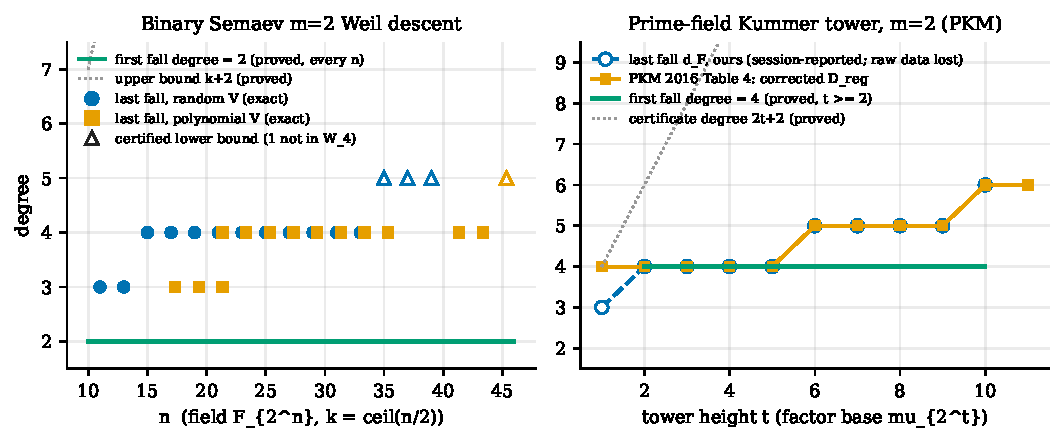
\includegraphics[width=\linewidth]{figures/fig-fall-degrees.pdf}
\caption[]{\emph{Left:} binary Semaev $m=2$ descent. The first fall degree
is 2 (Corollary~\ref{cor:ffd2}, proved). Filled marks are exact last fall
degrees per unsatisfiable instance. Open triangles are certified lower
bounds $d_{\tilde F}\ge5$ (Theorem~\ref{thm:lfd5}). The dotted line is the
proved upper bound $k+2$. \emph{Right:} prime-field Kummer tower, $m=2$
(\S\ref{sec:fd-pkm}). The session-reported last fall degree lies on the
corrected degree of regularity of PKM 2016, Table~4. The first fall degree
is 4 (proved). Values and sources: \art{figures/data-new.json}.}
\label{fig:fd}
\end{figure}

\begin{theorem}[Exact last fall degrees; computer-verified on instances]\label{thm:lfdexact}
On the diagonal $k=\lceil n/2\rceil$:
\begin{itemize}
\item $d_{\tilde F}=3$ on all six random-subspace instances at $n=11,13$
  and on all ten polynomial-subspace instances at $n=17,19$;
\item $d_{\tilde F}=4$ on all 29 random-subspace instances with
  $15\le n\le33$, and on all 25 polynomial-subspace instances with
  $23\le n\le35$ or $n=41,43$;
\item $d_{\tilde F}=4$ on Semaev's own cell ($n=40$, $k=20$, uniform $z$),
  matching his reported $d_{F4}=4$;
\item $d_{\tilde F}=5$ exactly on instance R35a ($n=35$, $k=18$, random
  $V$): $1\notin W_4$, and both restrictions $a_1=0,1$ are refuted at
  $W_4$ (Lemma~\ref{lem:branch}).
\end{itemize}
\end{theorem}

Table~\ref{tab:fd-binary} gives every instance behind
Theorems~\ref{thm:lfdexact} and~\ref{thm:lfd5}, one row per subspace family
and $n$, in the layout of Kousidis and Wiemers' Table~1.

\begin{table}[p]
\centering\small
\begin{tabular}{@{}clrrrrrrrr@{}}
\toprule
$m$ & $V$ & $n$ & $k$ & inst. & $D_{\rm ff}$ & $d_{\tilde F}$ & cols at $D=4$ & s at $D=4$ & codim $W_4\ge$ \\
\midrule
2 & P & 17 & 9 & 6 & 2 & 3 &  &  &  \\
 &  & 19 & 10 & 4 & 2 & 3 &  &  &  \\
 &  & 21 & 11 & 4 & 2 & 3$\times$2, 4$\times$2 & 9{,}109 & 7.3 &  \\
 &  & 23 & 12 & 4 & 2 & 4 & 12{,}951 & 7.3 &  \\
 &  & 25 & 13 & 4 & 2 & 4 & 17{,}902 & 11.1 &  \\
 &  & 27 & 14 & 4 & 2 & 4 & 24{,}158 & 20.3 &  \\
 &  & 29 & 15 & 3 & 2 & 4 & 31{,}931 & 40.9 &  \\
 &  & 31 & 16 & 3 & 2 & 4 & 41{,}449 & 51.9 &  \\
 &  & 33 & 17 & 3 & 2 & 4 & 52{,}956 & 100.1 &  \\
 &  & 35 & 18 & 2 & 2 & 4 & 66{,}712 & 160.9 &  \\
 &  & 41 & 21 & 1 & 2 & 4 & 124{,}314 & 1076.1 &  \\
 &  & 43 & 22 & 1 & 2 & 4 & 149{,}986 & 2001.3 &  \\
 &  & 45 & 23 & 1 & 2 & $\ge5$ & 179{,}447 & 1850.7 & 12{,}742 \\
\addlinespace
 & S & 40 & 20 & 2 & 2 & 4 & 102{,}091 & 537.9 &  \\
\addlinespace
 & R & 11 & 6 & 3 & 2 & 3 &  &  &  \\
 &  & 13 & 7 & 3 & 2 & 3 &  &  &  \\
 &  & 15 & 8 & 3 & 2 & 4 & 2{,}517 & 1.0 &  \\
 &  & 17 & 9 & 3 & 2 & 4 & 4{,}048 & 1.3 &  \\
 &  & 19 & 10 & 3 & 2 & 4 & 6{,}196 & 2.1 &  \\
 &  & 21 & 11 & 3 & 2 & 4 & 9{,}109 & 3.2 &  \\
 &  & 23 & 12 & 3 & 2 & 4 & 12{,}951 & 4.1 &  \\
 &  & 25 & 13 & 3 & 2 & 4 & 17{,}902 & 6.6 &  \\
 &  & 27 & 14 & 3 & 2 & 4 & 24{,}158 & 15.4 &  \\
 &  & 29 & 15 & 3 & 2 & 4 & 31{,}931 & 24.0 &  \\
 &  & 31 & 16 & 3 & 2 & 4 & 41{,}449 & 45.2 &  \\
 &  & 33 & 17 & 2 & 2 & 4 & 52{,}956 & 91.9 &  \\
 &  & 35 & 18 & 2 & 2 & $\ge5$ & 66{,}712 & 121.0 & 5{,}287 \\
 &  & 37 & 19 & 2 & 2 & $\ge5$ & 82{,}993 & 312.9 & 10{,}066 \\
 &  & 39 & 20 & 2 & 2 & $\ge5$ & 102{,}091 & 445.9 &  \\
\addlinespace
 & U & 33 & 17 & 2 & 2 & 4 & 52{,}956 & 95.4 &  \\
 &  & 35 & 18 & 2 & 2 & $\ge5$ & 66{,}712 & 126.4 & 5{,}287 \\
\addlinespace
 & T & 29 & 15 & 2 & 2 & 4 & 31{,}931 & 38.3 &  \\
 &  & 31 & 16 & 2 & 2 & 4 & 41{,}449 & 68.3 &  \\
 &  & 33 & 17 & 2 & 2 & $\ge5$ & 52{,}956 & 128.8 & 4{,}888 \\
\bottomrule
\end{tabular}

\caption[]{Binary Weil descent of $\Sem3$ ($m=2$, $k=\lceil n/2\rceil$): the
first fall degree $D_{\rm ff}=2$ (Corollary~\ref{cor:ffd2}, proved for
every $n$) beside the last fall degree $d_{\tilde F}$, the least $D$ with
$1\in W_D$, for each instance. Subspace families: P, Semaev's polynomial
subspace $\langle1,t,\ldots,t^{k-1}\rangle$; S, the same with uniform $z$
(Semaev's own cell); R, random; U, random with uniform $z$; T, random inside
$\ker\operatorname{Tr}$. ``$\ge5$'' means $1\notin W_4$; R35a is exactly 5
(Theorem~\ref{thm:lfdexact}). Columns: instances; columns of the degree-4 closure
matrix; median closure wall time at
$D=4$ in seconds, over the instances run to that degree (host not
recorded); certified codimension of $W_4$ where an independent certificate
was checked. Source:
\art{crypto-autoresearcher:analysis/semaev-m2-last-fall-degree/results/},
laid out by \art{figures/make_tab_fall_degrees.py} from
\art{figures/data-falldegree-instances.json}.}
\label{tab:fd-binary}
\end{table}

\begin{theorem}[Certified $d_{\tilde F}\ge5$]\label{thm:lfd5}
For each instance below, a certificate (Proposition~\ref{prop:cert}) for
$1\notin W_4(F)$ was accepted by the independent checker. Hence
$d_{\tilde F}\ge5$, and every F4 run reaches degree $\ge5$.

\smallskip\noindent
\begin{tabular}{@{}lllll@{}}
\toprule
instance & $n$ & $k$ & subspace & certified $\operatorname{codim}W_4\ge$ \\
\midrule
T33a, T33b & 33 & 17 & random $\subset K_0$ & 4{,}888 \\
R35a, R35b, U35a, U35b & 35 & 18 & random (U: uniform $z$) & 5{,}287 \\
Q35a, Q35b (satisfiable) & 35 & 18 & random & 5{,}287 \\
R37a, R37b & 37 & 19 & random & 10{,}066 \\
P45a & 45 & 23 & Semaev's default $\langle1,t,\ldots,t^{22}\rangle$ & 12{,}742 \\
C19a, C19b (chain $m=t=3$) & 19 & 7 & random & 9{,}253, 6{,}817 \\
\bottomrule
\end{tabular}

\smallskip\noindent
Two further instances, R39a and R39b ($n=39$), and C21a and C21b (the
chain at $n=21$) have $1\notin W_4$ by implementation~A alone.
\end{theorem}

For Q35a and Q35b, which have 6 and 2 Boolean solutions, the bound follows
from Proposition~\ref{prop:bridges}(4), since $5{,}287\gg|S|$. The P45a
closure stalls after three rounds at
$\dim W_4\cap B_{\le d}=(0,1,224,8950,166705)$, out of 179{,}447
monomials. Its quadratic part, $224=5n-1$, is exactly the
polynomial-subspace count of Lemma~\ref{lem:deg3}: at degree 4 the closure
finds no new falls.

\begin{corollary}[Semaev's Assumption 1 fails as stated]\label{cor:assump}
Semaev's Assumption~1~\cite[\S4.5]{semaev2015} asserts $d_{F4}\le4$ for
Boolean systems equivalent to his system (5), for $q=2^n$,
$k=\lceil n/m\rceil$, any subspace of dimension $k$ and any $2\le t\le m$.
Theorem~\ref{thm:lfd5} contradicts it in three cells:
\begin{itemize}
\item $(n,m,t,k)=(35,2,2,18)$, with random subspaces;
\item $(45,2,2,23)$, with his own default subspace;
\item $(19,3,3,7)$ and $(21,3,3,7)$, inside the parameter range of his
  tables, where his polynomial subspace gives 4 and random subspaces do
  not.
\end{itemize}
\end{corollary}

Table~\ref{tab:fd-chain} lists the chain instances. With Semaev's
polynomial subspace the closure refutes at degree~4 in every cell; with
random subspaces it does not at $n=19,21$.

\begin{table}[t]
\centering\small
\begin{tabular}{@{}lccrrlrrr@{}}
\toprule
instance & $m=t$ & $V$ & $n$ & $k$ & $d_{\tilde F}$ & cols at $D=4$ & s at $D=4$ & codim $W_4\ge$ \\
\midrule
D17a & 3 & P & 17 & 6 & $\le$4 & 59{,}536 & 294.6 &  \\
D17b & 3 & P & 17 & 6 & $\le$4 & 59{,}536 & 297.4 &  \\
D19a & 3 & P & 19 & 7 & $\le$4 & 102{,}091 & 1283.7 &  \\
D19b & 3 & P & 19 & 7 & $\le$4 & 102{,}091 & 1047.1 &  \\
D21a & 3 & P & 21 & 7 & $\le$4 & 124{,}314 & 1270.3 &  \\
D21b & 3 & P & 21 & 7 & $\le$4 & 124{,}314 & 1225.4 &  \\
C17a & 3 & R & 17 & 6 & $\le$4 & 59{,}536 & 281.3 &  \\
C17b & 3 & R & 17 & 6 & $\le$4 & 59{,}536 & 270.9 &  \\
C19a & 3 & R & 19 & 7 & $\ge$5 & 102{,}091 & 1088.5 & 9{,}253 \\
C19b & 3 & R & 19 & 7 & $\ge$5 & 102{,}091 & 1184.4 & 6{,}817 \\
C21a & 3 & R & 21 & 7 & $\ge$5 & 124{,}314 & 1806.2 &  \\
C21b & 3 & R & 21 & 7 & $\ge$5 & 124{,}314 & 1790.4 &  \\
\bottomrule
\end{tabular}

\caption[]{Chained system, $m=t=3$, $k=\lceil n/3\rceil$: closure at $D=4$
per instance. ``$\le4$'' means $1\in W_4$; ``$\ge5$'' means $1\notin W_4$.
Certified codimensions as in Table~\ref{tab:fd-binary}; C21a and C21b have
no checked certificate: $1\notin W_4$ by implementation~A alone. Source:
\art{crypto-autoresearcher:analysis/semaev-m2-last-fall-degree/results/instances_t3.json}.}
\label{tab:fd-chain}
\end{table}

\paragraph{What is new, and what is not.} That the degree of regularity
reaches 5 has been \emph{observed} before:
\begin{itemize}
\item Kosters and Yeo saw Magma step degrees of $\ge5$ at $n=40$ and
  $n=45$~\cite{kosters2015notes};
\item Kousidis and Wiemers saw F4 at step degree 5 for $n=37$--$48$, $m=2$,
  and wrote that a lower bound on the degree of regularity ``can
  potentially answer an open question''~\cite{kousidis2019}.
\end{itemize}
Table~\ref{tab:fd-kw} sets their $m=2$ rows beside ours at the same
$n$. The quantities differ: $D_{\rm reg}$ is the highest step degree of
their F4 runs, while $d_{\tilde F}$ is the closure degree of the system,
and no F4 run refutes below it. So their $5$ at $n=41,43$ against our $4$
on polynomial subspaces is not a contradiction; F4 overshoots the closure
there. At $n=35$ their $D_{\rm reg}=4$ agrees with our polynomial subspace
and differs from every random subspace we drew, which are all $\ge5$:
which subspace a table uses decides the degree it reports. At $n=45$ both
reach 5.

\begin{table}[t]
\centering\small
\begin{tabular}{@{}rrrrrrcc@{}}
\toprule
\multicolumn{6}{c}{Kousidis--Wiemers, Table 1 ($m=2$, F4)} & \multicolumn{2}{c}{this work, $d_{\tilde F}$} \\
\cmidrule(r){1-6}\cmidrule(l){7-8}
$n$ & $n'$ & $D_{\rm ff}$ & $D_{\rm reg}$ & s & GB & P or S & R, U or T \\
\midrule
34 & 17 & 2 & 4 & 188 & 1.2 &  &  \\
35 & 18 & 2 & 4 & 1{,}237 & 16.1 & 4 & $\ge5$$^{\rm R}$; $\ge5$$^{\rm U}$ \\
36 & 18 & 2 & 4 & 1{,}342 & 16.4 &  &  \\
37 & 19 & 2 & 5 & 2{,}542 & 29.2 &  & $\ge5$$^{\rm R}$ \\
38 & 19 & 2 & 5 & 2{,}815 & 25.2 &  &  \\
39 & 20 & 2 & 5 & 4{,}785 & 45.6 &  & $\ge5$$^{\rm R}$ \\
40 & 20 & 2 & 5 & 4{,}858 & 46.3 & 4$^{\rm S}$ &  \\
41 & 21 & 2 & 5 & 7{,}930 & 65.3 & 4 &  \\
42 & 21 & 2 & 5 & 8{,}901 & 66.7 &  &  \\
43 & 22 & 2 & 5 & 16{,}816 & 95.5 & 4 &  \\
44 & 22 & 2 & 5 & 15{,}690 & 96.8 &  &  \\
45 & 23 & 2 & 5 & 38{,}352 & 140.0 & $\ge5$ &  \\
46 & 23 & 2 & 5 & 31{,}735 & 140.7 &  &  \\
47 & 24 & 2 & 5 & 103{,}200 & 207.7 &  &  \\
48 & 24 & 2 & 5 & 86{,}636 & 208.2 &  &  \\
\bottomrule
\end{tabular}

\caption[]{The $m=2$ rows of Kousidis and Wiemers' Table~1~\cite{kousidis2019}
(F4, averages over ten repetitions; $n'=\lceil n/2\rceil$; time in
seconds, memory in GB), transcribed from the published table, beside the
last fall degree of our instances at the same $n$
(Table~\ref{tab:fd-binary}). Superscripts give the subspace family. Their
$m=3,4$ rows ($D_{\rm ff}=D_{\rm reg}=7$ and $13$, $n\le21$) concern
$\Sem4$ and $\Sem5$ and have no counterpart here.}
\label{tab:fd-kw}
\end{table}

Those are properties of solver runs. Theorem~\ref{thm:lfd5} is a property
of the systems, carried by a certificate any reader can check. With
Corollary~\ref{cor:ffd2} it makes the separation between first and last
fall degree rigorous on named instances. What remains open is the same
as before: a proof that $d_{\tilde F}\to\infty$. Semaev's asymptotics
survive if the regularity degree is $o(\sqrt{n\ln n})$, so only a growing
lower bound bears on the subexponential claim.

\paragraph{Re-verification.} For this treatise, the T33a certificate was
regenerated from the committed producer (M4RI 20200125, 4\,min 40\,s on
4~vCPUs) and checked with \texttt{cert\_check.py}:
\begin{itemize}
\item the certificate is byte-identical to the recorded SHA-256
  \texttt{cf9dcae8\ldots22cf};
\item the checker reports ``1 is not in $W_4(F)$, and
  $\operatorname{codim}W_4(F)\ge4888$'' (38.8\,s);
\item the closure dimensions $(0,0,64,2968,48068)$ match the record.
\end{itemize}
Source: \art{research/paper_opportunities_20261029/REPORT.md}, \S6.

\section{Explicit membership over any field: the guarded chain}\label{sec:fd-guarded}

A second presentation encodes factor-base membership directly. Let $S$ be
a set of $B$ abscissae of rational points, and $g(T)=\prod_{s\in S}(T-s)$.
The two-$\Sem3$ chain with an inverse guard is
\[
  F_S=\{g(x),\ g(y),\ g(z),\ \Sem3(x,y,u),\ \Sem3(u,z,r),\ v(x-y)-1\},
\]
with $r=x(R)$. Degrees are ordinary total degrees with explicit inputs.
The first fall degree is the homogeneous-top syzygy degree modulo Koszul
syzygies. Source: \art{research/guarded_fall_degree_20261028/}, which holds
written proofs, independent audits, a native exact replay and partial
Lean.

\begin{theorem}[Guarded chain]\label{thm:guarded}
For unsatisfiable instances:
\begin{enumerate}
\item Short Weierstrass curves, $p>3$, $B=3$:
  $(d_{\rm ff},d_F)=(4,5)$, \emph{exactly}, for every $p$.
\item Same presentation, any $B\ge3$: $d_{\rm ff}=B+1$ and
  $\max(5,B+1)\le d_F\le3B-4$.
\item Ordinary binary curves $Y^2+XY=X^3+a_2X^2+a_6$, $B=3$:
  \begin{itemize}
  \item $d_F=4$ if and only if $g=T^3+c$, which is possible only for even
    $n$;
  \item $d_F=5$ otherwise.
  \end{itemize}
  So for odd $n$, which covers every SEC~2 binary size, every
  unsatisfiable instance has $(4,5)$.
\item Binary curves, $B\ge4$: $B+1\le d_F\le3B-4$.
\end{enumerate}
\end{theorem}

\begin{proof}[Proof sketch of (1)]
\emph{Upper bound.} The divided difference
$Q=(g(x)-g(y))/(x-y)$ enters $V_4$ through the guard. The pair is then
replaced by the missing root $w=s_1-x-y$. The two quadratics in $u$ are
normalised and their resultant extracted in stages inside $V_5$. Finally
the unit $T(w,z)$ is inverted in $K[w,z]/(g(w),g(z))\cong K^9$.

\emph{Lower bound.} The space $W=(I_0\cap R_{\le4})+Kf_1+Kf_2$ is closed
under the degree-4 operations and excludes 1. This uses characteristic
$>3$, through $-3\ne0$.
\end{proof}

Exact degree-5 refutation DAGs were replayed in native arithmetic on public
fixtures:
\begin{itemize}
\item $p=101$ and $p=5$;
\item secp256k1, P-256, P-384 and P-521, with $S=\{x(G),x(2G),x(4G)\}$ and
  $R=16G$; the DAGs have 413--415 nodes, and OpenSSL rechecks the points.
\end{itemize}
Twenty polynomial identities used in the proofs are checked in Lean
(\texttt{FallDegreeIdentities.lean}, \texttt{PrimeBitLocal.lean}; axioms
\texttt{propext} and \texttt{Quot.sound} only). The degree-4 lower bound
is now machine-checked: \texttt{GuardedModel.no\_degree\_four\_refutation}
proves that 1 is not derivable at degree four from the six generators, over
every field with $6\ne0$ and three distinct base abscissae, and
\texttt{lastFall\_lower} states the last-fall consequence under an explicit
unit-ideal hypothesis (\art{research/guarded_fall_degree_20261028/formal/GuardedModel.lean};
six modules, fresh \texttt{leanchecker} replays and a transitive axiom audit,
merged in \#2814). The degree-5 upper construction, the bridge from rational
unsatisfiability to the unit ideal, and the first-fall syzygy statement are
\emph{not} formalised, so the exact pair $(4,5)$ is not yet a Lean theorem. A
\texttt{lastFallDegree} definition and Caminata--Gorla's Theorem~2.8 in
\art{crypto-autoresearcher:formal/CryptoResearch/FallDegree/LastFall.lean}
are the bridge a complete formalisation would build on.

Two Boolean upper bounds accompany the guarded chain:
\begin{itemize}
\item $d_F\le3\ell+1$ for the fully Boolean binary encoding, with $\ell$
  bits per base coordinate;
\item $d_F\le3\ell+2$ for a prime-field bit-restricted lookup encoding.
\end{itemize}
Both are instances of the standard brute-force refutation in Polynomial
Calculus~\cite{cei1996}: fix the base bits, and refute the affine residue.
For the binary chain at $t=3$ they are weaker than Theorem~\ref{thm:upper}'s
$2k+3$.

\section{Prime-field Kummer towers}\label{sec:fd-pkm}

Petit, Kosters and Messeng~\cite{pkm2016} take the factor base
$V=\mu_{2^t}$ over $\FF_p$ (with $2^t\mid p-1$). They write membership as a
tower $y_0=x/g$, $y_{j+1}=y_j^2$, $y_{t-1}^2=1$, and argue the complexity
from the first fall degree. Source for this section:
\art{research/prime_fall_degree_20261027/DERIVED.md}, written proofs D1--D8.

\begin{theorem}[Kummer towers, $m=2$]\label{thm:pkm}
Let $R=\FF_p[y]/T$ be the tower quotient. Items (3)--(5) concern
\emph{inconsistent} systems, those whose reduced $\Sem3$ is a unit of $R$; a
satisfiable target has no inverse in $R$, and the refutation bounds do not
apply to it.
\begin{enumerate}
\item $T$ is a Gröbner basis, and $R\cong\FF_p^{V^m}$. So every ideal
  over $R$ is radical, and an $m=2$ system is inconsistent if and only if
  the reduced $\Sem3$ is a unit of $R$.
\item $R=\FF_p[z]/(z^K-1)$ with $K=2^t$. The degree of a monomial $z^k$ is
  $\operatorname{popcount}(k)$, and degree falls are exactly binary
  carries.
\item If $t\ge2$, $g\ne0$, $3x_R^2+a\ne0$ and the system is inconsistent, then $d_{\rm ff}=4$
  (operational convention), for every $t$. The degree-2 part of $f$ is a
  bilinear form with $\det M=-2g^6(3x_R^2+a)\ne0$, so nothing falls at 3;
  the monomial $q=y_{10}y_{11}$ gives a fall at 4.
\item For an inconsistent system, the no-fall certificate has degree
  $d_F\le2+\operatorname{popdeg}(f^{-1})\le2t+2$.
\item For an inconsistent system in the naive presentation
  $\{\Sem3,\ x_i^K-g^K\}$ of the \emph{same} set, $d_F\ge2^t$. So $d_F$ is not an invariant of the ideal; it depends
  on the presentation.
\item A single summand has $d_F=2$ for every $t$. Growth at $m=2$ must
  therefore come from the genus-one curve $f(z_1,z_2)=0$; no
  specialisation to finitely many points can show it.
\end{enumerate}
\end{theorem}

\paragraph{Measured, and prior.} Table~\ref{tab:fd-pkm} sets the study's
session-reported median last fall degree for $t=1..10$ at
$p=2{,}013{,}265{,}921$ beside the corrected degree of regularity in PKM's
own Table~4 for $n_1=1..11$ (also Figure~\ref{fig:fd}, right). The raw
records were never committed (the study's \texttt{RESTART.md}), so the
$d_F$ column is session-reported, not re-derivable. From $t=2$ on the two
columns coincide.

\begin{table}[t]
\centering\small
\begin{tabular}{@{}rrrr@{}}
\toprule
$t$ (PKM: $n_1$) & $D_{\rm ff}$ (proved) & $d_F$ (session median) & PKM $D_{\rm reg}^{\rm corr}$ \\
\midrule
1 &  & 3 & 4 \\
2 & 4 & 4 & 4 \\
3 & 4 & 4 & 4 \\
4 & 4 & 4 & 4 \\
5 & 4 & 4 & 4 \\
6 & 4 & 5 & 5 \\
7 & 4 & 5 & 5 \\
8 & 4 & 5 & 5 \\
9 & 4 & 5 & 5 \\
10 & 4 & 6 & 6 \\
11 &  &  & 6 \\
\bottomrule
\end{tabular}

\caption[]{Prime-field Kummer tower, $m=2$, factor base $\mu_{2^t}$:
the proved first fall degree (Theorem~\ref{thm:pkm}(3); it needs $t\ge2$),
the session-reported median last fall degree at $p=2{,}013{,}265{,}921$
(raw data not committed), and the corrected degree of regularity
$D_{\rm reg}^{\rm corr}$ of Petit, Kosters and Messeng, Table~4
(prime case)~\cite{pkm2016}. Source: \art{figures/data-new.json}, from
\art{research/prime_fall_degree_20261027/}.}
\label{tab:fd-pkm}
\end{table} So the \emph{growth} is prior art. What
Theorem~\ref{thm:pkm} adds is the proved constant first fall degree beside
it, and the presentation dependence. A prediction,
$d_F=4+\lfloor(t-2)/4\rfloor$, was registered before any $t\ge11$ row and
is untested.

\section{Measured solving degrees in other presentations}

The binary programme measured refutation and closure degrees on many
presentations; the full record is in~\cite[\S6]{icprogram2026}.
Table~\ref{tab:fd-other} lists the last fall degree by base-subspace
dimension $\ell$. It is flat in $n$ at fixed $(m,\ell)$ and rises with
$\ell$.

\begin{table}[t]
\centering\small
\begin{tabular}{@{}rrcc@{}}
\toprule
$m$ & $\ell$ & $n$ & $d_F$ \\
\midrule
3 & 5 & 10--15 & 4 \\
  & 6 & 16--24 & 4 \\
  & 7 &        & $\ge5$ (every draw) \\
\addlinespace
4 & 3 & 9--14  & 4 \\
\addlinespace
5 & 3 & 11--15 & 4 \\
\bottomrule
\end{tabular}
\caption[]{Binary decomposition systems in other presentations: last fall
degree $d_F$ by $m$ and base-subspace dimension $\ell$, over the measured
range of $n$. At $(m,\ell)=(3,7)$ every draw is refuted only at degree
$\ge5$. Source:~\cite[\S6]{icprogram2026}.}
\label{tab:fd-other}
\end{table}

Three further measurements bear on the solver rather than the system:
\begin{itemize}
\item \emph{Plain refutation tracks the semi-regular degree.} The plain
  Macaulay refutation degree stays within one of the semi-regular
  prediction in all 14 exact cells.
\item \emph{Closure algorithms refute one or two degrees earlier.} A
  MutantXL-style closure refutes all 92 unsatisfiable draws at degree 3--4,
  where XL needs 5--7.
\item \emph{Guessing variables restores degree 4.} Fixing one or two
  variables restores degree 4 at $(m,\ell)=(3,7)$, at $1/116$--$1/260$ of
  the projected degree-5 cost.
\end{itemize}
Every observed growth is growth in the size of the factor base: in $\ell$,
$k$, $t$, $B$, or the digit count $s$ of a prime digit presentation (where
$d_{\rm ff}=d_F=4+\lfloor s/2\rfloor$ at $m=2$, reproduced by a curve-free
null). None was observed in $n$ at a fixed base.

\section{What this settles and what it does not}\label{sec:fd-summary}

\begin{itemize}
\item \emph{Settled.} In the three presentations the programme studied,
  the first fall degree is a proved constant of the presentation: 2 for
  binary Weil descent, $B+1$ for explicit membership, 4 for Kummer
  towers. The last fall degree is not bounded by it.
  \begin{itemize}
  \item This is proved for the guarded chain at $B=3$ (exactly 5 against
    4).
  \item It is certified on named binary instances: $\ge5$ against 2, at
    $n=33$--$45$ and in the $m=t=3$ chain.
  \item It is measured for Kummer towers (6 against 4 at $t=10$).
  \end{itemize}
  Any complexity argument that substitutes the first fall degree for the
  solving degree is unsupported for these systems.
\item \emph{Not settled.} No presentation has a proved last-fall lower
  bound that grows with $n$. That is the open problem of
  HKY~\cite{hky2015} and Kousidis--Wiemers~\cite{kousidis2019}, and the
  only result that would bear on the subexponential claims. The upper
  bounds $k+2$ and $(t-1)k+t$ are linear in $n$, far above every observed
  value.
\item \emph{Missing before submission.} The certificates are committed
  only as hashes; they regenerate (above) but need public hosting. The
  sample is small: two instances per $n$ at $n\ge33$, one polynomial
  instance at $n\ge41$. The written proofs need expert review. The
  Kummer-tower data must be regenerated
  (\art{research/paper_opportunities_20261029/}).
\end{itemize}
